\documentclass[a4paper,indent]{paper}
\usepackage{tikz}
\usepackage{microtype}
\usepackage{inputenc}
\usepackage{rotating}
\usepackage{fullpage}
\usepackage{caption}
\usepackage{tikz}
\usepackage{tikz-timing}
\usepackage{mdframed}
\usepackage{fourier} % for /danger
\usepackage{amsmath}
\usepackage{acronym}
\usepackage[hidelinks]{hyperref}

\usetikzlibrary{arrows, shapes.gates.logic.US, calc}
%\usetikzlibrary{external} % doesn't work with tikz timing diagrams
%\tikzexternalize % activate!

\title{Auger Radio Digitizer}
\subtitle{Software and interfaces}
\author{%
  Sjoerd T. Timmer (s.timmer@astro.ru.nl)\\
  Roel Jordans (r.jordans@astro.ru.nl)}
\date{}


\acrodef{RD}[RD]{Radio Digitizer}
\acrodef{UUB}[UUB]{Universal Upgrade Board}
\acrodef{SPI}[SPI]{Serial Peripheral Interface}
\acrodef{ADC}[ADC]{analog-to-digital converter}
\acrodef{FPGA}[FPGA]{field programmable gate array}
\acrodef{DDR}[DDR]{double data rate}
\acrodef{GPIO}[GPIO]{general-purpose IO}
\acrodef{LNA}[LNA]{low-noise amplifier}
\acrodef{PGA}[PGA]{programmable-gain amplifier}
\acrodef{MSB}[MSB]{most-significant bit}
\acrodef{I2C}[$\text{I}^2\text{C}$]{}
\acused{I2C}
%\newmdenv[linecolor=orange,backgroundcolor=orange!10]{warning}

\newenvironment{warning}
{\par\begin{mdframed}[linewidth=2pt,linecolor=orange,backgroundcolor=orange!10]%
    \begin{list}{}{\leftmargin=0mm}\item[\bf\danger{}~~Warning: ]}
  {\end{list}\end{mdframed}\par}

\begin{document}
\maketitle{}
\begin{abstract}
  This document describes the internal firmware architecture of the Auger \acf{RD} module and the external interface to the \acs{UUB} board.  \acresetall
\end{abstract}

\tableofcontents

\clearpage


\section{Physical interface}
The Auger \ac{RD} module is connected to the \ac{UUB} with a 25-pin D-sub connector.
On the \ac{UUB} side this connects to a 24-pin JST B24B, or SAMTEC STMM-112-01-S-D connector.
The interface pins contain 8 differential (LVDS) pairs for data and multiple power (+24V) and ground points.
Half of the 8 data signals carry the radio data traces and the other 4 are dedicated to the housekeeping interface:%

\begin{tabular}{llllllll}
  %\shortstack{UUB\\fpga\\pin} &%
  \shortstack{UUB\\schema\\name} &%
  \shortstack{JST B24B\\(old connector)} &%
  \shortstack{SAMTEC\\STMM-112\\-01-S-D(new)} &%
  \shortstack{D-sub\\pin} &%
  \shortstack{RD schema\\name} &%
  \shortstack{RD fpga\\pin} &%
  \shortstack{pin\\function}
  \\\hline
  EXTn\_P\_D1 & 1   & 2  & 1  & LVDS\_0+  & L4 & SPI MOSI\\
  EXTn\_N\_D1 & 2   & 1  & 14 & LVDS\_0-  & L5 &  \\
  EXTn\_P\_D0 & 3   & 4  & 2  & LVDS\_1+  & J3 & SPI CLK \\
  EXTn\_N\_D0 & 4   & 3  & 15 & LVDS\_1-  & K3 &  \\
  GND         & 5   & 6  & 3  & GND       &    &  \\
  24V         & 6   & 5  & 16 & 24V       &    &  \\
  EXTn\_P\_D2 & 7   & 8  & 4  & LVDS\_2+  & K2 & DATA 0 \\
  EXTn\_N\_D2 & 8   & 7  & 17 & LVDS\_2-  & J1 &  \\
  EXTn\_P\_D4 & 9   & 10 & 5  & LVDS\_3+  & M4 & DATA 1 \\
  EXTn\_N\_D4 & 10  & 9  & 18 & LVDS\_3-  & N5 &  \\
  GND         & 11  & 12 & 6  & GND       &    &  \\
  24V         & 12  & 11 & 19 & 24V       &    &  \\
  EXTn\_P\_D3 & 13  & 14 & 7  & LVDS\_4+  & G2 & DATA CLK \\
  EXTn\_N\_D3 & 14  & 13 & 20 & LVDS\_4-  & F1 &  \\
  EXTn\_P\_D5 & 15  & 16 & 8  & LVDS\_5+  & N4 & SPI CE \\
  EXTn\_N\_D5 & 16  & 15 & 21 & LVDS\_5-  & P5 &  \\
  GND         & 17  & 18 & 9  & GND       &    &  \\
  24V         & 18  & 17 & 22 & 24V       &    &  \\
  EXTn\_P\_D6 & 19  & 20 & 10 & LVDS\_6+  & P3 & TRIGGER \\
  EXTn\_N\_D6 & 20  & 19 & 23 & LVDS\_6-  & P4 &  \\
  EXTn\_P\_D7 & 21  & 22 & 11 & LVDS\_7+  & N2 & SPI MISO \\
  EXTn\_N\_D7 & 22  & 21 & 24 & LVDS\_7-  & M1 &  \\
  GND         & 23  & 24 & 12 & GND       &    &  \\
  24V         & 24  & 23 & 25 & 24V       &    &  \\
              &     &    & 13 & GND or NC &    &  \\
\end{tabular}
\captionof{table}{\acs{RD} pin configuration.}

\begin{center}
  \begin{minipage}[b]{0.2\textwidth}
    \centering
    \includegraphics[height=4cm]{img/images-000.png}
  \end{minipage}
  \begin{minipage}[b]{0.5\textwidth}
    \centering
    \includegraphics[height=6cm]{img/images-002.png}
  \end{minipage}
  \begin{minipage}[b]{0.2\textwidth}
    \centering
    \includegraphics[height=4cm]{img/images-004.png}
  \end{minipage}
  \begin{minipage}[t]{0.2\textwidth}
    \centering
    \captionof{figure}{D-sub}
  \end{minipage}
  \begin{minipage}[t]{0.5\textwidth}
    \centering
    \captionof{figure}{JST B24B}
  \end{minipage}
  \begin{minipage}[t]{0.2\textwidth}
    \centering
    \captionof{figure}{SAMTEC\\STMM-112\\-01-S-D}
  \end{minipage}
\end{center}

\subsection{Front panel}
TODO

\subsection{Status LEDs}
The leds are permanently on as soon as the RD is successfully booted.
\begin{warning}
  This behaviour is planned to change in the future. 
\end{warning}



\section{Software interface}
The Auger \ac{RD} module has two separate interfaces.
One fast interface to capture radio traces, and one slower \ac{SPI} interface for housekeeping and metadata. 

\subsection{Radio data}
The Auger \ac{RD} module samples 12-bit data from 2 channels at 250 Msamples/s into a circular buffer.
It does so continuously until it sees a rising edge on the trigger input.
When the trigger is received the \ac{RD} will continue to write a configurable number of post-trigger samples to the buffer.
The number of pre-trigger and post-trigger samples can be configured using the housekeeping \ac{SPI} interface and defaults to 1024/1024 at power-up.
See Section \ref{sec:trigger_offset} for details. The total buffer always contains 2048 samples.

When the post-trigger samples have been recorded, the transfer is automatically initiated.
Figures~\ref{fig:datatransferstart}~and~\ref{fig:datatransferfinish} show the data transfer protocol. 
The transfer is clocked from the RD at 60 MHz. The clock is held high outside the transmission windows.
\begin{warning}
  The 60 MHz speed is subject to change. Due to the distribution of events, a 1\% reduction in transfer time would increase the number of recorded events by 5\%.
\end{warning}
The transmission starts with a preamble consisting of 3 rising clock edges.
After the preamble, the 2048 samples are transmitted. Data for the 2 channels is separately transmitted on the 2 data lines.
Each sample is shifted out, most significant bit first, followed by a parity bit (odd parity). Finally, 11 trailing clock cycles are transmitted.

\begin{center}
  \begin{minipage}[b]{\textwidth}
    \centering
    %\includegraphics[width=\textwidth]{img/data-transfer-start.pdf}
    \begin{tikztimingtable}[timing/wscale=1.2]
      clk     & HHLCCCCCCCCCCCCCCCCCCCCCCCCCCCCCCCCCCCCCCCCCCCC \\ 
      data[0] & UUUUUUUUDDDDDDDDDDDDDDDDDDDDDDDD{Sample 0 Channel 0 [11:0]}DD{parity}DDDDDDDDDDDDD{Sample 1 Channel 0 [11:0]} \\
      data[1] & UUUUUUUUDDDDDDDDDDDDDDDDDDDDDDDD{Sample 0 Channel 1 [11:0]}DD{parity}DDDDDDDDDDDDD{Sample 1 Channel 1 [11:0]} \\
    \end{tikztimingtable}
    \captionof{figure}{Start of data transfer has 3 leading clock edges. Data is stable at rising edges. Parity bit follows data.}\label{fig:datatransferstart}
  \end{minipage}\vspace{\baselineskip}
  \begin{minipage}[b]{\textwidth}
    \centering
    %\includegraphics[width=\textwidth]{img/data-transfer-finish.pdf}
    \begin{tikztimingtable}[timing/wscale=1.2]
      clk     & CCCCCCCCCCCCCCCCCCCCCCCCCCCCCCCCCCCCCCCCHHHHHHH \\ 
      data[0] & DDDDDDDDDDDDDDDD{Sample 2047 Channel 0 [11:0]}DD{parity}UUUUUUUUUUUUUUUUUUUUUUUUUUUUU \\
      data[1] & DDDDDDDDDDDDDDDD{Sample 2047 Channel 1 [11:0]}DD{parity}UUUUUUUUUUUUUUUUUUUUUUUUUUUUU \\
    \end{tikztimingtable}
    
    \captionof{figure}{End of data transfer has 11 trailing rising edges.}\label{fig:datatransferfinish}
  \end{minipage}
\end{center}

There is negligeable delay between the registration of the last sample and the start of the transmission and between the end of the transmission and the registration of the first sample for the next trace.

During the transmission and during the recording of the pre-trigger samples the value of the trigger input is ignored.



\subsection{Jitter and latency}\label{sec:latency}
Data is transferred from an \ac{ADC} (ADS4229) to an \ac{FPGA} (Lattice ECP5 LFE5U-12F) over 12 LVDS pairs. The data transfer is \ac{DDR} which means that the even bits are transferred on the rising edges of the 250 MHz clock and the odd bits on the falling edges. In the \ac{FPGA} the \ac{DDR} data is decoded and further processed at 125 MHz. I.e., samples are processed 4 at a time (2 samples each from 2 channels). This means that triggers are also registered at the 125 MHz clock and that the RD inherently incurs an extra 1 sample jitter on the location of the trigger.
\begin{warning}
  This is subject to change. The planned next version will sample the trigger at 500 MHz and actually provide one additional bit of trigger location information that can recovered through the housekeeping.
\end{warning}


Using the trigger-offset feature of the \ac{SPI} housekeeping interface, the location of the data window relative to the trigger can be configured. By default the location is set to 1024. I.e. the center of the window. However, the trigger signal is synchronized to the 125 MHz clock domain using two registers. This results in 2 clock cycles delay (i.e. 4 samples).

The \ac{ADC} is also subject to 16 clock cycles latency (at 250 MHz). In total there are therefore 1036 or 1037 samples before the trigger and 1011 or 1012 samples after the trigger.

\begin{warning}
  An experiment is planned but not yet executed to verify if the 12 sample delay is correctly calculated and --in particular-- if the jitter of 1 additional clock cycle is applied correctly in the mentioned figures.
\end{warning}


\begin{center}
  \includegraphics[width=\textwidth]{img/rd_timing.pdf}
  \captionof{figure}{Timing of \ac{RD} capture.}\label{fig:rd_timing}
\end{center}

\subsection{\acs{SPI} housekeeping interface}

\subsubsection{General Architecture}
The \ac{SPI} interface exposes several features including: firmware updates, science \ac{ADC} re-configuration, \ac{GPIO} access, a temperature sensors, and readout of \ac{LNA}/bias status.
The latter provides operating voltages and currents independently on each channel.

All of the above features are handled by independent sub-systems that  are internally bridged by an \ac{SPI} demuxer. The first 8 bits of every \ac{SPI} transaction are captured by the demuxer. The remainder of the transaction is forwarded transparently to the sub-system in question.

An example program \texttt{rd\_housekeeping} is provided that exposes most of the available features. Refer to the source in the git repository\footnote{\url{https://github.com/auger-prime-sde/rd/tree/master/uub-linux-tools/rd_housekeeping}}.

\begin{center}
  \begin{tikztimingtable}
    clk                   & HH21{C} {[dotted]10{C}} 5{C}HH \\
    ce in                 & HH21{L} {[dotted]10{L}}5{L}HH \\
    mosi                  & UU16{D}{address, e.g. 0x06}5{D}[dotted]10{D}[solid]5{D}{forwarded data}UU \\    
    \ldots                & \\
    ce to sub-system 0x05 & 23{H} {[dotted]10{H}}7{H} \\
    ce to sub-system 0x06 & 18{H}5{L} {[dotted]10{L}} 5{L} 2{H} \\
    ce to sub-system 0x07 & 23{H} {[dotted]10{H}}7{H} \\
    \ldots                & \\
  \end{tikztimingtable}
  \captionof{figure}{\ac{SPI} demuxer example.}
\end{center}


\subsubsection{\acs{SPI} mode and speed}
The \ac{SPI} interface was tested upto 12 MHz. It is known that all sub-systems can also reach that speed.
The external interface operates with CPOL=1 and CPHA=1 (spi mode 3) at all times. The ADS4229 science adc operates in mode 2 but the responsible sub-system block handles the translation. All \ac{SPI} data is transferred \ac{MSB} first. 


\subsubsection{\ac{GPIO} (address 0x01)}
Eight \ac{GPIO} pins are available on the \ac{RD} board. All pins are configured as outputs. The \ac{GPIO} sub-system allows writing to and reading from the output buffer. The \ac{GPIO} cannot be configured as input pins. Each transaction exists of a command byte, optionally followed by a data byte in case of a write command.

The supported commands are:
\begin{center}
  \begin{tabular}{|l|l|l|}
    \hline
    command & code & expects data \\
    \hline
    read & 0x00 & no \\
    write & 0x01 & yes \\
    set bits (gpio = gpio | data) & 0x02 & yes \\
    clear bits (gpio = gpio \& $\neg{}$ data) & 0x03 & yes \\
    reset to default (0xFF) & 0x04 & no \\
    \hline
  \end{tabular}
  \captionof{table}{\ac{GPIO} commands.}
\end{center}

\begin{center}
  \begin{tikztimingtable}
    clk  & HHCCCCCCCCCCCCCCCCCCCCCCCCCCCCCCCCCCCCCCCCCCCCCCCCHH \\
    ce   & HHLLLLLLLLLLLLLLLLLLLLLLLLLLLLLLLLLLLLLLLLLLLLLLLLHH \\
    mosi & UUDDDDDDDDDDDDDDDD{0x01 (select \ac{GPIO})}DDDDDDDDDDDDDDDD{0x00 (\ac{GPIO} read)}UUUUUUUUUUUUUUUUUU \\
    miso & UUUUUUUUUUUUUUUUUUUUUUUUUUUUUUUUUUDDDDDDDDDDDDDDDD{0x42 (for example)}UU \\
  \end{tikztimingtable}
  \vspace{\baselineskip}\\
  \begin{tikztimingtable}
    clk  & HHCCCCCCCCCCCCCCCCCCCCCCCCCCCCCCCCCCCCCCCCCCCCCCCCHH \\
    ce   & HHLLLLLLLLLLLLLLLLLLLLLLLLLLLLLLLLLLLLLLLLLLLLLLLLHH \\
    mosi & UUDDDDDDDDDDDDDDDD{0x01 (select \ac{GPIO})}DDDDDDDDDDDDDDDD{0x01 (\ac{GPIO} write)}DDDDDDDDDDDDDDDD{0x00 (for example)}UU \\
    miso & UUUUUUUUUUUUUUUUUUUUUUUUUUUUUUUUUUDDDDDDDDDDDDDDDD{0x42 (old data)}UU \\
  \end{tikztimingtable}
  \captionof{figure}{Example \ac{GPIO} read and write. The output register contains the data 0x42 and is written to 0x00.}
\end{center}


\subsubsection{Program flash pass-through (address 0x02)}
Transactions to address 0x02 are forwarded transparently to the \ac{SPI} flash chip.
Refer to the SST26VF032B documentation for details.

\begin{center}
  \begin{tikztimingtable}[timing/wscale=0.6]
    clk      & HHCCCCCCCCCCCCCCCCCCCCCCCCCCCCCCCCCCCCCCCCCCCCCCCCCCCCCCCCCCCCCCCCCCCCCCCCCCCCCCCCHH \\
    uub ce   & HHLLLLLLLLLLLLLLLLLLLLLLLLLLLLLLLLLLLLLLLLLLLLLLLLLLLLLLLLLLLLLLLLLLLLLLLLLLLLLLLLHH \\
    flash ce & HHHHHHHHHHHHHHHHHHLLLLLLLLLLLLLLLLLLLLLLLLLLLLLLLLLLLLLLLLLLLLLLLLLLLLLLLLLLLLLLLLHH \\
    mosi     & UUDDDDDDDDDDDDDDDD{0x02 (select \ac{SPI} flash)}DDDDDDDDDDDDDDDD{0x9F (read id)}UUUUUUUUUUUUUUUUUUUUUUUUUUUUUUUUUUUUUUUUUUUUUUUUUU \\
    miso     & UUUUUUUUUUUUUUUUUUUUUUUUUUUUUUUUUUDDDDDDDDDDDDDDDD{0xBF}DDDDDDDDDDDDDDDD{0x26}DDDDDDDDDDDDDDDD{0x42}UU\\
  \end{tikztimingtable}
  \captionof{figure}{Example SST26VF032B JEDEC-ID readout.}
\end{center}



\subsubsection{Science adc pass-through (address 0x03)}
The science \ac{ADC} has a \ac{SPI} configuration interface. The ADS4229 expects \ac{SPI} mode 2 (cpol=1, cpha=0) but also works in \ac{SPI} mode 1 (cpol=0, cpha=1) which is achieved by inverting the clock signal from the \ac{UUB} interface.

\begin{center}
  \begin{tikztimingtable}[timing/wscale=1]
    uub spi clk & HHCCCCCCCCCCCCCCCCCCCCCCCCCCCCCCCCCCCCCCCCCCCCCCCCHH \\
    uub spi ce  & HHLLLLLLLLLLLLLLLLLLLLLLLLLLLLLLLLLLLLLLLLLLLLLLLLHH \\
    mosi        & UUDDDDDDDDDDDDDDDD{0x03 (select ADS4229 adc)}DDDDDDDDDDDDDDDD{0x25 (gain register)}DDDDDDDDDDDDDDDD{0x40 gain setting}UU \\
    adc spi ce  & HHHHHHHHHHHHHHHHHHLLLLLLLLLLLLLLLLLLLLLLLLLLLLLLLLHH \\
    adc spi clk & LLLLLLLLLLLLLLLLLLCCCCCCCCCCCCCCCCCCCCCCCCCCCCCCCCLL \\
  \end{tikztimingtable}
  \captionof{figure}{Example ADS4229 transaction. This sets the channel A gain (config register address 0x25) to 2dB.}
\end{center}




\subsubsection{ADS1015 current and voltage sensors (address 0x04)}
\begin{warning}
  The exact control of the ADS1015 and Si7060 is under debate and subject to change.
\end{warning}

The ADS1015 is a four port \ac{I2C} \ac{ADC} which is wired to measure the voltage and the current on both \ac{LNA} channels. This can be used to determine if the \ac{LNA} is properly connected and working as expected.

Whenever a rising edge on the trigger input is received, the controller for this \ac{I2C} chip will execute a fixed sequence of \ac{I2C} commands and store the conversion result in a register. The register can be read via \ac{SPI} and contains eight bytes:

\begin{center}
  \begin{tabular}{|l|l|}
    \hline
    Register address & contents \\
    \hline
    0x00 & bits [11:4] of \acs{ADC} channel 0 (N/S bias current)\\
    0x01 & bits [3:0]  of \acs{ADC} channel 0, followed by four zeroes\\
    0x02 & bits [11:4] of \acs{ADC} channel 1 (N/S bias voltage)\\
    0x03 & bits [3:0]  of \acs{ADC} channel 1, followed by four zeroes \\
    0x04 & bits [11:4] of \acs{ADC} channel 2 (E/W bias current)\\
    0x05 & bits [3:0]  of \acs{ADC} channel 2, followed by four zeroes \\
    0x06 & bits [11:4] of \acs{ADC} channel 3 (E/W bias voltage)\\
    0x07 & bits [3:0]  of \acs{ADC} channel 3, followed by four zeroes \\
    \hline
  \end{tabular}
  \captionof{table}{ADS1015 register layout}
\end{center}

Upon receiving a trigger, the \ac{RD} delays the readout of the \ac{I2C} devices until all science data has been written to the internal buffer. This is done to avoid polution of the spectrum. After completion of the write phase, but before initiating the science data transfer, the 4 ADS1015 conversions are started. Because the ADS1015 makes one \ac{ADC} conversion at a time the samples are not made in parallel but sequentially. Due to the maximum sampling frequency of the ADS1015 (3300 SPS) the \ac{RD} has to stall for 315 ns after each conversion. 
All four conversions take 2.16 ms in total to complete. If another trigger is received in that time it does not cause another readout but rather assumes that the previously read values are still correct. Note that is such cases the \ac{I2C} communication may overlap with the start of the next data acquisition phase.

The ADS1015 has a \ac{PGA}. All conversions are made with the $FSR=\pm4.096 V$ setting. I.e. $MSB = 2 mV$.

To read a byte from the register, write the address of that register and read the data on the next byte. The next address can already be written during the read and therefore the whole register can efficiently be retrieved in a 10-byte transaction (including the sub-system address byte).

\begin{center}
  \begin{tikztimingtable}[timing/wscale=0.8]
    clk  & HHCCCCCCCCCCCCCCCCCCCCCCCCCCCCCCCCCCCCCCCCCCCCCCCCCCCCCCCCCCCCCCCCHH \\
    ce   & HHLLLLLLLLLLLLLLLLLLLLLLLLLLLLLLLLLLLLLLLLLLLLLLLLLLLLLLLLLLLLLLLLHH \\
    mosi & UUDDDDDDDDDDDDDDDD{0x04 (select ADS1015)}DDDDDDDDDDDDDDDD{0x04}DDDDDDDDDDDDDDDD{0x05}UUUUUUUUUUUUUUUUUU \\
    miso & UUUUUUUUUUUUUUUUUUUUUUUUUUUUUUUUUUDDDDDDDDDDDDDDDD{$I_{E/W}[11:4]$}DDDDDDDD{$I_{E/W}[3:0]$}DDDDDDDD{0000}UU \\
  \end{tikztimingtable}
  \captionof{figure}{Example ADS1015 register readout for the E/W \ac{LNA} bias current.}
\end{center}


\subsubsection{SI7060 temperature sensor (address 0x05)}
\begin{warning}
  The exact control of the ADS1015 and Si7060 is under debate and subject to change.
\end{warning}

The Si7060 is an \ac{I2C} temperature sensor which measures the temperature inside the \ac{RD} enclosure.

Whenever a rising edge on the trigger input is detected, the controller for this \ac{I2C} chip will execute a fixed sequence of \ac{I2C} commands and stores the conversion result in a register. The register can be read via \ac{SPI} and contains two bytes:

\begin{center}
  \begin{tabular}{|l|l|}
    \hline
    Register address & contents \\
    \hline
    0x00 & Dspsigm of Si7060 (one status bit and data bits [14:8])\\
    0x01 & Dspsigl of Si7060 (data bits [7:0])\\
    \hline
  \end{tabular}
  \captionof{table}{ADS1015 register layout.}
\end{center}

Upon receiving a trigger, the \ac{RD} delays the readout of the \ac{I2C} devices until all science data has been written to the internal buffer. This is done to avoid polution of the spectrum. After completion of the write phase, but before initiating the science data transfer, the Si7060 temperature conversion and readout is started.

The entire readout including conversion takes 0.2475 ms in total to complete. If another trigger is received in that time it does not cause another readout but rather assumes that the previously read values are still correct.

The raw 15-bit data is calculated as:
$$
D =  \text{Dspsigm}[6:0] < < 8 + \text{Dspsigl}[7:0]
$$

The temperature can be calculated as follows:
$$
T (^\circ{}C) = 55 + (D - 16384) / 160
$$



To read a byte from the register simply write the address of that register and read the data on the next byte. The next address can already be written during the read and therefore the whole register can efficiently be read in one 4-bute transaction (including the sub-system address byte).

\begin{center}
  \begin{tikztimingtable}[timing/wscale=0.8]
    clk  & HHCCCCCCCCCCCCCCCCCCCCCCCCCCCCCCCCCCCCCCCCCCCCCCCCCCCCCCCCCCCCCCCCHH \\
    ce   & HHLLLLLLLLLLLLLLLLLLLLLLLLLLLLLLLLLLLLLLLLLLLLLLLLLLLLLLLLLLLLLLLLHH \\
    mosi & UUDDDDDDDDDDDDDDDD{0x05 (select Si7060)}DDDDDDDDDDDDDDDD{0x00}DDDDDDDDDDDDDDDD{0x01}UUUUUUUUUUUUUUUUUU \\
    miso & UUUUUUUUUUUUUUUUUUUUUUUUUUUUUUUUUUDDDDDDDDDDDDDDDD{Dspsigm}DDDDDDDDDDDDDDDD{Dspsigl}UU \\
  \end{tikztimingtable}
  \captionof{figure}{Example Si7060 temperature readout.}
\end{center}







\subsubsection{Version info (address 0x07)}
This sub-system will always return a 1-byte version code.
The currently known version codes are:
\begin{center}
  \begin{tabular}{|l|l|}
    \hline
    Code & Description \\
    \hline
    0x00 & legacy (version info not implemented) \\
    0x01, 0x02 & used during development \\
    0x03 & version shipped with \ac{RD} v3 units for the Malargue engineering array in November 2019\\
    \hline
  \end{tabular}
\end{center}

\begin{center}
  \begin{tikztimingtable}[timing/wscale=0.8]
    clk  & HH32{C}HH \\
    ce   & HH32{L}HH \\
    mosi & UU16{D}{0x07 (select version)}16{U}UU \\
    miso & UU16{U}16{D}{0x03 (version code)}UU \\
  \end{tikztimingtable}
  \captionof{figure}{Example version read.}
\end{center}






\subsubsection{Trigger-offset configuration(address 0x08)}\label{sec:trigger_offset}
The position of the trigger within the data window can be configured.
This trigger-offset is set to 1024 (mid window) on power up but can be changed using this interface.
The value is set by writing two bytes to this sub-system. Only the lower 11 bits are used. The upper 5 bits are ignored.
The written number represents the position in the data trace where the trigger will be located. Note that the actual trigger appears at a slightly different position due to latency in the \ac{ADC} and in the \ac{RD}. Refer to Figure~\ref{fig:rd_timing} for details.
\begin{center}
  \begin{tikztimingtable}[timing/wscale=1]
    clk  & HHCCCCCCCCCCCCCCCCCCCCCCCCCCCCCCCCCCCCCCCCCCCCCCCCHH \\
    ce   & HHLLLLLLLLLLLLLLLLLLLLLLLLLLLLLLLLLLLLLLLLLLLLLLLLHH \\
    mosi & UUDDDDDDDDDDDDDDDD{0x08 (select offset reg)}UUUUUUUUUUDDDDDD{offset[11:8]}DDDDDDDDDDDDDDDD{offset[7:0]}UU \\
  \end{tikztimingtable}
  \captionof{figure}{Example start-offset setting transaction.}
\end{center}


\subsubsection{Boot time and boot sequence}
After power is applied the \ac{FPGA} loads its configuration from the SST26VF032B \ac{SPI} flash.
As soon as the user code is running the \ac{RD} executes a hard-coded initialization sequence on the \ac{SPI} interface, as if the \ac{UUB} had sent the following commands:

\begin{center}
  \begin{tabular}{|l|l|}
    \hline
    \acs{SPI} commands & Description \\
    \hline
    \texttt{0x03 0x00 0x02} & ADS4229 software reset \\
    \texttt{0x03 0x29 0x00} & re-assert default configuration \\
    \texttt{0x03 0x41 0x00} & re-assert default configuration \\
    \texttt{0x03 0x03 0x03} & enable high-performance mode \\
    \texttt{0x03 0xF2 0x00} & disable low speed mode (already off by default)\\
    \texttt{0x03 0xEF 0x00} & disable low speed mode (already off by default)\\
    \texttt{0x03 0x41 0x00} & cmos mode off (already off by default)\\
    \texttt{0x03 0x02 0x40} & enable high performance mode \\
    \texttt{0x03 0xD5 0x18} & enable high performance mode \\
    \texttt{0x03 0xD7 0x0C} & enable high performance mode \\
    \texttt{0x03 0xDB 0x20} & enable high performance mode \\
    \texttt{0x08 0x04 0x00} & set trigger-offset to 1024 \\
    \hline
  \end{tabular}
  \captionof{table}{\ac{RD} initialization sequence. }
  
\end{center}

This initialization sequences takes approximately 170 us. During this time the \ac{SPI} lines from the \ac{UUB} are inhibited and the MISO line will remain silent.




\section{Developers Guide/Architecture}
\subsection{General architecture}
\subsubsection{\acs{SPI} demux}

\subsubsection{Boot sequence injection}


\subsection{Housekeeping sub-systems}

\subsubsection{Program flash (0x02)}

\subsubsection{Science \acs{ADC} (0x03)}

\subsubsection{Current and voltage monitoring (0x04)}

\subsubsection{Temperature sensor (0x05)}

\subsubsection{Trigger injection (0x06)}

\subsubsection{Firmware version register (0x07)}

\subsubsection{Trigger-offset register (0x08)}

\subsection{\acs{ADC} driver}
The adc\_driver converts the 12 \ac{DDR} 250 MHz data lines to 48 `normal' data lines at 125MHz.
At each clock cycle 2 samples are produced for each of the 2 channels.
In the ADS4229 datasheet we find that the bits of the samples are organized as follows:
\begin{center}
  \begin{tabular}{l|l|l}
    \acs{RD} schema name & ADS4229 name & timing \\
    \hline
    250 MHz clk&      & \texttiming[timing/wscale=5,timing/initchar=H]{LHL0.04H}\\
    \\
    D0  & DA0  & \texttiming[timing/wscale=5]{uD{ch0 bit 0}D{ch0 bit 1}u}\\
    D1  & DA2  & \texttiming[timing/wscale=5]{uD{ch0 bit 2}D{ch0 bit 3}u}\\
    D2  & DA4  & \texttiming[timing/wscale=5]{uD{ch0 bit 4}D{ch0 bit 5}u}\\
    D3  & DA6  & \texttiming[timing/wscale=5]{uD{ch0 bit 6}D{ch0 bit 7}u}\\
    D4  & DA8  & \texttiming[timing/wscale=5]{uD{ch0 bit 8}D{ch0 bit 9}u}\\
    D5  & DA10 & \texttiming[timing/wscale=5]{uD{ch0 bit 10}D{ch0 bit 11}u}\\
    \\
    D6  & DB0  & \texttiming[timing/wscale=5]{uD{ch1 bit 0}D{ch1 bit 1}u}\\
    D7  & DB2  & \texttiming[timing/wscale=5]{uD{ch1 bit 2}D{ch1 bit 3}u}\\
    D8  & DB4  & \texttiming[timing/wscale=5]{uD{ch1 bit 4}D{ch1 bit 5}u}\\
    D9  & DB6  & \texttiming[timing/wscale=5]{uD{ch1 bit 6}D{ch1 bit 7}u}\\
    D10 & DB8  & \texttiming[timing/wscale=5]{uD{ch1 bit 8}D{ch1 bit 9}u}\\
    D11 & DB10 & \texttiming[timing/wscale=5]{uD{ch1 bit 10}D{ch1 bit 11}u}\\
  \end{tabular}
  \captionof{figure}{Organization of samples on the \ac{DDR} lines.}
\end{center}

The (auto generated) adc\_driver outputs the bits in a different layout (i.e. grouped by arrival time):


\begin{center}
  \begin{tikztimingtable}[timing/wscale=3]
    250 MHz clk         & [H]LHLHL0.04H\\
    125 MHz clk         & L2H2L0.04H\\
    RD-D0  ADS4229-DA0  & uD{q[0] }D{q[13]}D{q[26]}D{q[39]}u\\
    RD-D1  ADS4229-DA2  & uD{q[1] }D{q[14]}D{q[27]}D{q[40]}u\\
    RD-D2  ADS4229-DA4  & uD{q[2] }D{q[15]}D{q[28]}D{q[41]}u\\
    RD-D3  ADS4229-DA6  & uD{q[3] }D{q[16]}D{q[29]}D{q[42]}u\\
    RD-D4  ADS4229-DA8  & uD{q[4] }D{q[17]}D{q[30]}D{q[43]}u\\
    RD-D5  ADS4229-FA10 & uD{q[5] }D{q[18]}D{q[31]}D{q[44]}u\\
    RD-D6  ADS4229-DB0  & uD{q[6] }D{q[19]}D{q[32]}D{q[45]}u\\
    RD-D7  ADS4229-DB2  & uD{q[7] }D{q[20]}D{q[33]}D{q[46]}u\\
    RD-D8  ADS4229-DB4  & uD{q[8] }D{q[21]}D{q[34]}D{q[47]}u\\
    RD-D9  ADS4229-DB6  & uD{q[9] }D{q[22]}D{q[35]}D{q[48]}u\\
    RD-D10 ADS4229-DB8  & uD{q[10]}D{q[23]}D{q[36]}D{q[49]}u\\
    RD-D11 ADS4229-FB10 & uD{q[11]}D{q[24]}D{q[37]}D{q[50]}u\\
    trigger             & uD{q[12]}D{q[25]}D{q[38]}D{q[51]}u\\
  \end{tikztimingtable}
  \captionof{figure}{Adc\_driver output format.}
\end{center}


Note that the trigger input is used as the 13th input to the \ac{DDR} decoder.
This provides four synchonized samples of the trigger input.
The last sample (q[51]) is used to trigger the write\_controller.
The second (q[25]) is used to determine if the even or odd sample will be used as the first (and last) sample in the trace.
The sub-sample trigger information (q[12] \textbf{xor} q[25] \textbf{xor} q[36]) can be retrieved through the housekeeping \ac{SPI} interface.

\begin{warning}
  This behaviour has not yet been implemented.
  The current implementation simply forwards the external trigger to the write\_controller which samples it as 125 MHz with minimal synchonization.
\end{warning}





\subsubsection{Write Controller}
%The write controller is responsible for enabling and disabling writes to the circular buffer.
%It listens in on the address counter ($i\_curr\_address$) and controls (besides the write enable ($o\_write\_enable$)) the start ($o\_trigger\_done$) and trigger-offset ($o\_start\_addr$) of the Readout Controller.
%
%A configurable trigger-offset ($i\_start\_offset$) determines how many samples are stored before the trigger.
%In the current instantiation the address width is eleven bits so there are 2048 samples and therefore $2048 - i\_start\_offset$ samples after the trigger.
%
%
%The Write Controller needs to be enabled with a pulse on the $i\_arm$ input.
%After this pulse the Write Controller will enable writes within 2 clock cycles.
%
%The \ac{ADC} driver outputs 2 samples in each clock cycle (for each channel, so 4 in total at each clock cycle).
%Therefore the Write Controller should wait for at least
%$$
%\left\lceil\frac{i\_start\_offset}{2}\right\rceil
%$$
%clock cycles  before accepting triggers.
%
%After the trigger is first seen high, the Write Controller should keep $o\_write\_enable$ high for exactly
%$$
%\left\lceil\frac{2048 - i\_start\_offset}{2}\right\rceil
%$$
%clock cycles. At that time $o\_write\_enable$ has to be asserted low and $o\_trigger\_done$ should be asserted high. At that time $o\_start\_addr$ has to be set to the address at which the data starts:
%$$
%i\_curr\_addr - i\_start\_offset \pmod{2048}
%$$
%This condition should hold until the next pulse on the $i\_arm$ signal.
%
%
%A trigger-offset of 0 (or 1) is considered invalid but anything in the closed interval $[1, 2047]$ should work.
%



\subsubsection{Trigger injection through housekeeping \ac{SPI}}
\begin{warning}
  This \ac{SPI} sub-system is candidate for removal in the next release.
  This address 0x06 may become a trigger for the \ac{I2C} readout instead.
\end{warning}

There is an \ac{SPI} sub-system at address 0x06 that can be used to trigger the \ac{RD} if no external trigger is present.
This is useful for debugging.
The inverted CE of this submodule is or'ed with the external trigger input. It is not necessary to send any data for the trigger to work.
\begin{center}
  \begin{tikztimingtable}[timing/wscale=1]
    clk    & HHCCCCCCCCCCCCCCCCHH \\
    ce     & HHLLLLLLLLLLLLLLLLHH \\
    mosi   & UUDDDDDDDDDDDDDDDD{0x06 (internal trigger)}UU \\
    trig\_int & HHHHHHHHHHHHHHHHHLHH \\
  \end{tikztimingtable}
  \captionof{figure}{Example transaction to inject an internal trigger.}
\end{center}
\begin{center}
  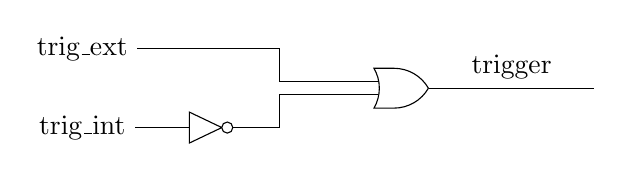
\begin{tikzpicture}
    \node (te) at (0, 1) {trig\_ext};
    \node (ti) at (0, 0) {trig\_int};
    \node[not gate US, draw] at ($(ti) + (1.5, 0)$) (notti) {};
    \node[or gate US, draw, rotate=0, logic gate inputs=nn] at ($(notti) + (2.5, 0.5)$) (teornotti) {};
    \draw (ti) -- (notti.input);
    \draw (te) -- (2.5,1) |- (teornotti.input 1);
    \draw (notti.output) -- (2.5,0) |- (teornotti.input 2);
    \draw (teornotti.output) -- node[above]{trigger} ($(teornotti) + (2.5, 0)$);
  \end{tikzpicture}
  \captionof{figure}{Internal wiring of internal and external trigger.}
\end{center}





\end{document}